\documentclass[11pt]{beamer}

\usepackage[utf8]{inputenc}
\usepackage[T1]{fontenc}

% Graphics
\usepackage{graphicx}
\usepackage{tikz}

% Language localization
\usepackage[english]{babel}

% Symbols
\usepackage{amsmath}
\usepackage{amsfonts}
\usepackage{amssymb}

% Bold math style, useful for vectors
\usepackage{bm}

\usepackage{ulem}

\usetheme{Madrid}
\setbeamertemplate{navigation symbols}{}

\begin{document}
	\author{Niklas Wingren}
	\title{Acousto-electromagnetic interaction}
	\subtitle{An overview focused on non-destructive testing}
	\date{October 11, 2018}
	\frame[plain]{\maketitle}
	
	\begin{frame}{Contents}
		\tableofcontents
	\end{frame}
	
	\section{Background}
	\begin{frame}{Background}{Non-destructive testing}
		
	\end{frame}
	
	\begin{frame}{Background}{Interaction mechanisms}
		\begin{itemize}
			\item Boundary perturbation of discrete objects
			\item Localized harmonic motion inside object
			\item Photoelastic interaction
			\item Displacement of scatterers by acoustic wave
		\end{itemize}
	\end{frame}
	
	\begin{frame}{Background}{Interaction mechanisms}
		\begin{itemize}
			\item \sout{Boundary perturbation of discrete objects}
			\item Localized harmonic motion inside object
			\item Photoelastic interaction
			\item \sout{Displacement of scatterers by acoustic wave}
		\end{itemize}
	\end{frame}
	
	\section{Localized harmonic motion}
	\begin{frame}{Localized harmonic motion}{Generating localized harmonic motion}
		
	\end{frame}
	
	\begin{frame}{Localized harmonic motion}{Micro-Doppler effect}
		
	\end{frame}
	
	\begin{frame}{Localized harmonic motion}{Harmonic motion microwave Doppler imaging (HMMDI)}
		
	\end{frame}
	
	\section{Photoelastic interaction}
	\begin{frame}{Photoelastic interaction}{Acousto-optics}
		\begin{columns}
		\begin{column}{0.4\textwidth}
			\resizebox{\textwidth}{!}{
				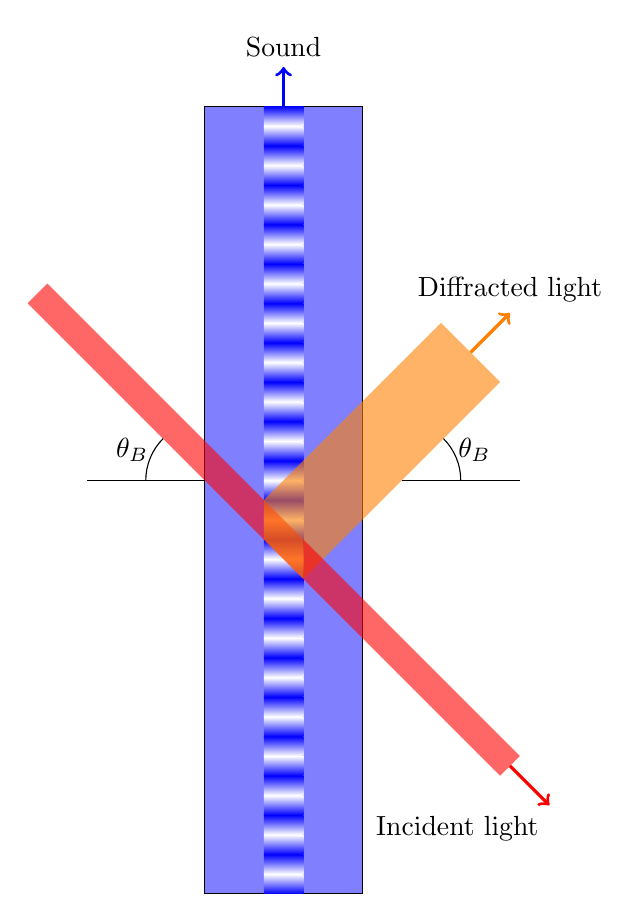
\begin{tikzpicture}[scale=0.5]
					\draw[fill=blue!50!white] (-2,0) rectangle ++(4,20);
					\foreach \i in {0,1,...,39}
						\path [bottom color=blue, top color=white, shading angle = {mod(\i,2)*180}]
						(-0.5,{\i/2}) rectangle ++(1,0.5);
						
					\fill[red,opacity=0.6] (-6.5,15) -- ++(7,-7) -- (0.5,9) -- ++({-7+sqrt(0.5-0.5*0.5)},7-0.5);
					\fill[orange,opacity=0.6] (0.5,8) -- ++(5,5) -- ++({-sqrt(4.5-1.5*1.5)},1.5) -- (-0.5,10) -- (-0.5,9);
					\fill[red,opacity=0.6] (0.5,8) -- ++(5,-5) -- ++({sqrt(0.5-0.5*0.5)},0.5) -- (0.5,9);
					
					\draw[->,blue,very thick] (0,20) -- (0,21) node[anchor=south,text=black]{Sound};
					\draw[->,orange,very thick] ({5.5-sqrt(4.5-1.5*1.5)+sqrt(1.5*1.5/2-0.75*0.75)},13.75) -- ++(1,1) node[anchor=south,text=black]{Diffracted light};
					\draw[->,red,very thick] ({5.5+sqrt(0.5-0.5*0.5)-sqrt(0.5*0.5/2-0.25*0.25)},3.25) -- ++(1,-1) node[anchor=north east,text=black]{Incident light};
					
					\draw (-2,10.5) -- ++(-3,0);
					\draw[shift={(-2,10.5)}] ([shift={(180:1.5)}] 0,0) arc(180:135:1.5) (157.5:2) node{$\theta_B$};
					\draw (3,10.5) -- ++(3,0);
					\draw[shift={(3,10.5)}] ([shift={(0:1.5)}] 0,0) arc(0:45:1.5) (22.5:2) node{$\theta_B$};
				\end{tikzpicture}
			}
		\end{column}
		\begin{column}{0.6\textwidth}
			\begin{equation*}
				\sin{\theta_B} = \frac{\lambda}{2\Lambda}
			\end{equation*}
		\end{column}
		\end{columns}
	\end{frame}
	
	\begin{frame}{Photoelastic interaction}{Photoelasticity}
		\begin{itemize}
			\item Tensor relation between strain and change in relative permittivity
			\begin{equation*}
				\Delta \varepsilon_{r_i} = -\varepsilon_{r_i}^2 p_{ij} S_j
			\end{equation*}
			\item Relation to standard tensor notation for a quantity $x$
			\begin{align*}
				x_1 &= x_{11},\ x_2 = x_{22},\ x_3 = x_{33}, \\
				x_4 &= x_{23},\ x_5 = x_{31},\ x_6 = x_{12}
			\end{align*}
			\item $p_{ij}$ can have 36 independent components, but for isotropic solids it simplifies to
			\begin{align*}
				p_{11} &= p_{22} = p_{33}, \ p_{12} = p_{21} = p_{13} = p_{23} = p_{32}\\
				p_{44} &= p_{55} = p_{66} = \frac{1}{2} (p_{11} - p_{22}), \ p_{ij} = 0 \text{ for others}
			\end{align*}
		\end{itemize}
	\end{frame}
	
	\begin{frame}{Photoelastic interaction}{Photoelasticity}
		\begin{itemize}
			\item Anisotropy in $\varepsilon_r$ arises even in isotropic solids
			\begin{itemize}
				\item $\varepsilon_r$ depends on $p_{11}$ parallel to, and $p_{12}$ perpendicular to acoustic axis
			\end{itemize}
			\item If  $p_{11} \approx p_{12}$ a scalar approximation is
			\begin{equation*}
				\Delta \varepsilon_r(x,t) = -\mathfrak{p} \varepsilon_r^2 s(x,t), \quad \mathfrak{p} = \frac{p_{11} + p_{12}}{2}
			\end{equation*}
			\item A very simplistic model for $\mathfrak{p}$ based on the Lorentz-Lorenz relation is
			\begin{equation*}
				\mathfrak{p} = -\frac{(\varepsilon_r - 1)(\varepsilon_r + 2)}{3\varepsilon_r^2}
			\end{equation*}
		\end{itemize}
	\end{frame}
		
	\begin{frame}{Photoelastic interaction}{Scattering against dielectric perturbation}
		\begin{itemize}
			\item Time dependence related to incident fields separated
			\begin{align*}
				&\bm{\mathcal{E}}(\bm{r},t) = \bm{E}(\bm{r},t) \text{e}^{-i\omega t} \\
				&\bm{\mathcal{H}}(\bm{r},t) = \bm{H}(\bm{r},t) \text{e}^{-i\omega t} \\
			\end{align*}
			\item Maxwell's equations
			\begin{align*}
				&\nabla \times \bm{E} = i\omega \mu_0 \bm{H} - \mu_0 \frac{\partial \bm{H}}{\partial t} \\
				&\nabla \times \bm{H} = -i\omega \varepsilon \bm{E} + \mu_0 \frac{\partial (\varepsilon \bm{E})}{\partial t} \\
				&\nabla \cdot (\varepsilon \bm{E}) = 0 \\
				&\nabla \cdot \bm{H} = 0
			\end{align*}
		\end{itemize}
	\end{frame}
		
	\begin{frame}{Photoelastic interaction}{Scattering against dielectric perturbation}
		\begin{itemize}
			\item Definition for a small dielectric perturbation $\varepsilon_1$
			\begin{equation*}
				\varepsilon = \varepsilon_0(\varepsilon_r + \varepsilon_1)
			\end{equation*}
			\item Approximate equation for the electric field
			\begin{equation*}
				\nabla^2\bm{E} + k^2 \bm{E} =
				-k^2 \frac{\varepsilon_1}{\varepsilon_r} \bm{E} -\frac{1}{\varepsilon_r}\nabla(\bm{E} \cdot \nabla \varepsilon_1)
			\end{equation*}
			\item Scattering integral for weak scattering
			{\footnotesize \begin{equation*}
				\bm{E}_{sc}(\bm{r},t) = \frac{1}{4\pi\varepsilon_r} \int_{V_{sc}} \frac{e^{ik |\bm{r}-\bm{r'}| }}{ |\bm{r}-\bm{r'}|} \left( k^2 \bm{E}_i (\bm{r'},t) \varepsilon_1 (\bm{r'},t) + \nabla (\bm{E}_i (\bm{r'},t) \cdot \nabla \varepsilon_1 (\bm{r'},t)) \right) \mathrm{d}v'
			\end{equation*}}
		\end{itemize}
	\end{frame}
	
	\begin{frame}{Photoelastic interaction}{Simple scattering geometry}
		\resizebox{!}{0.6\textheight}{
			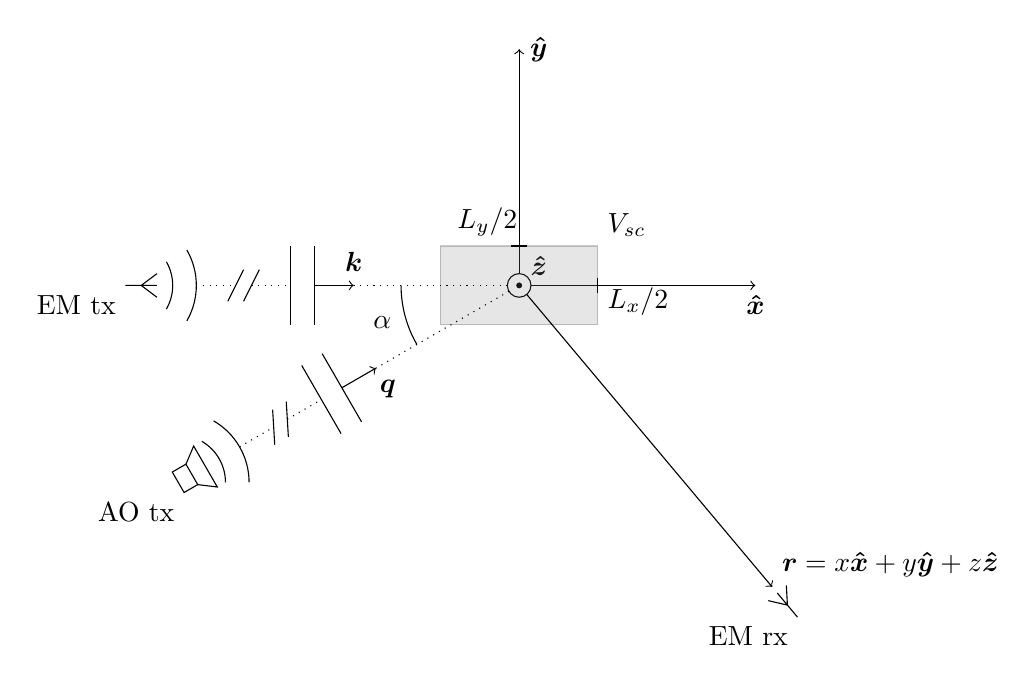
\begin{tikzpicture}
			% Draw coordinate axes
			\draw (0,0) circle(0.15);
			\filldraw[black] circle(0.03);
			\draw[->] (0.15,0) -- (3,0);
			\draw[->] (0,.150) -- (0,3);
			\draw (3,-0.25) node{$\bm{\hat{x}}$} (0.25,3) node{$\bm{\hat{y}}$} (0.25,0.25) node{$\bm{\hat{z}}$};
			
			% Draw scattering cube (or rectangle in this case)
			\draw[fill=gray,opacity=0.2] (-1,-0.5) rectangle(1,0.5);
			\draw (1,-0.1) -- (1,0.1) node[anchor= north west]{$L_x/2$} (-0.1,0.5) -- (0.1,0.5) node[anchor= south east]{$L_y/2$} (1,0.5) node[anchor=south west]{$V_{sc}$};
			
			% Draw EM tx and spherical waves
			\draw[shift = {(-5,0)}] (0,0) node[anchor=north east]{EM tx} -- (0.4,0) (0.2,0) -- (0.4,0.15)
			(0.2,0) -- (0.4,-0.15);
			\draw[shift = {(-5,0)}] ([shift={(-30:0.6)}] 0,0) arc(-30:30:0.6) ([shift={(-30:0.9)}] 0,0) arc(-30:30:0.9);
			
			% Draw EM "long distance" lines
			\draw[shift = {(-4.1,0)},dotted] (0,0) -- (0.5,0) (0.7,0) -- (1.2,0);
			\draw[shift = {(-4.1,0)}] (0.4,-0.2) -- (0.6,0.2) (0.6,-0.2) -- (0.8,0.2);
			
			% Draw EM plane waves
			\draw[shift = {(-2.9,0)}] (0,-0.5) -- (0,0.5) (0.3,-0.5) -- (0.3,0.5);
			\draw[shift = {(-2.6,0)}, ->] (0,0) -- (0.5,0);
			\draw[shift = {(-2.6,0)}] (0.5,0.3) node{$\bm{k}$};
			\draw[dotted] (-0.15,0) -- (-2.1,0);
			
			% Draw AO tx and spherical waves
			\draw[shift = {(210:5)}, rotate = 30] (0,-0.15) node[anchor=north east]{AO tx} rectangle (0.2,0.15) -- (0.4,0.3) -- (0.4,-0.3) -- (0.2,-0.15);
			\draw[shift = {(210:5)}, rotate = 30] ([shift={(-30:0.6)}] 0,0) arc(-30:30:0.6) ([shift={(-30:0.9)}] 0,0) arc(-30:30:0.9);
			
			% Draw AO "long distance" lines
			\draw[shift = {(210:4.1)}, rotate = 30,dotted] (0,0) -- (0.5,0) (0.7,0) -- (1.2,0);
			\draw[shift = {(210:4.1)}, rotate = 30] (0.4,-0.2) -- (0.6,0.2) (0.6,-0.2) -- (0.8,0.2);
			
			% Draw AO plane waves
			\draw[shift = {(210:2.9)}, rotate = 30] (0,-0.5) -- (0,0.5) (0.3,-0.5) -- (0.3,0.5);
			\draw[shift = {(210:2.6)}, rotate = 30, ->] (0,0) -- (0.5,0);
			\draw[shift = {(210:2.6)}, rotate = 30] (0.5,-0.3) node{$\bm{q}$};
			\draw[rotate = 30, dotted] (-0.15,0) -- (-2.1,0);
			
			% Draw angle alpha
			\draw ([shift={(180:1.5)}] 0,0) arc(180:210:1.5) (195:1.8) node{$\alpha$};
			
			% Draw line towards receiver
			\draw[->] (310:0.15) -- (310:5) node[anchor=south west]{$\bm{r} = x\bm{\hat{x}} + y\bm{\hat{y}} + z\bm{\hat{z}}$};
			
			% Draw EM rx
			\draw[shift = {(310:5.5)}, rotate = 130] (0,0) node[anchor=north east]{EM rx} -- (0.4,0) (0.2,0) -- (0.4,0.15) (0.2,0) -- (0.4,-0.15);
			\end{tikzpicture}
		}
		
		Fields close to the scattering center:
		\begin{align*}
			\bm{E}_i (\bm{r}',t) &= \bm{E}_i (\bm{r}') = \bm{E}_{i0} e^{i\bm{k}\cdot\bm{r}'} \\
			\varepsilon_1 (\bm{r}',t) &= -\mathfrak{p} \varepsilon_r^2 S_0 \cos(\bm{q} \cdot \bm{r}' - \Omega t)
		\end{align*}
	\end{frame}
	
	\begin{frame}{Photoelastic interaction}{Radar equation}
		\begin{equation*}
			\textit{SNR}^\pm_N = \frac{P_T R_T G_R \lambda_R^2 \sigma^\pm (\theta,\phi)}{(4\pi)^3 R_T^2 R_R^2 kT_0 B \cdot \mathit{NR}} N
		\end{equation*}
		\small
		\begin{equation*}
			\sigma^\pm (\theta, \phi) = \frac{\varepsilon_r^2 k^4}{16\pi} \mathfrak{p}^2 S_0^2 L_x^2 L_y^2 L_z^2 \Phi^\pm (\theta,\pi)^2
		\end{equation*}
		\begin{multline*}
			\Phi^\pm(\theta,\phi) = \text{sinc} \left( \frac{L_x}{2\pi} \left( k - k\sin{\theta}\cos{\phi} \pm q\cos{\alpha} \right) \right) \\
			\cdot \text{sinc} \left( \frac{L_y}{2\pi} \left( -k\sin{\theta}\sin{\phi} \pm q\sin{\alpha} \right) \right) 
			\text{sinc} \left( -\frac{L_z}{2\pi} k\cos{\theta} \right)
		\end{multline*}
	\end{frame}
	
	\begin{frame}{Photoelastic interaction}{Geometry for maximum scattering}
		\begin{equation*}
			\begin{cases}
				\theta = \pi/2 \\
				\cos{\alpha} = \mp \frac{q}{2k} = \mp \frac{\lambda}{2\Lambda} \\
				\tan{\frac{\phi}{2}} = \pm \sqrt{\frac{q^2}{4k^2-q^2}} = \pm \sqrt{\frac{\lambda^2}{4\Lambda^2-\lambda^2}}
			\end{cases}
		\end{equation*}
	\end{frame}
	
\end{document}